\documentclass{report}
\usepackage[utf8]{inputenc}
\usepackage{graphicx}
\usepackage[siunitx ,europeanresistors ,americaninductors]{circuitikz}
\usepackage{tikz}
\usepackage{pgfplots}
\graphicspath{{images/}}

\title{”Vienkāršu elektrisku shēmu modelēšana”}
\author{Pāvels Bitko}
\date{May 2018}

\begin{document}

\maketitle

\chapter{Teorētiskā daļa}
\section{Ķēdes aprēķins}

171REB165 

\begin{circuitikz}[scale=1, every node/.style={transform shape}]
\draw
(0,2) to[V=$V1$, ] (0,0)
(0,2) to[R=$R1$, -] (4,2)
(4,2) to[R=$R2$, -] (4,0)
(0,0) to[short, -] (4,0)
;
\end{circuitikz}

\begin{flushleft}
V1 = 165/10 = 16.5 V

R1 = 6+1 = 7 Ohm

R2 = 5+1 = 6 Ohm 
\end{flushleft}

Lai aprēķināt spriegumu uz R2 vajag izmantot sprieguma dalītāja formulu. \cite{gramata1} \cite{gramata2}
\begin{flushleft}
I = V1/(R1+R2) = 16.5/(6+7) = 1.27 A

UR1 = I*R1 = 7*1.27 = 8.88 V

UR2 = I*R2 = 6*1.27 = 7.61 V 

No šīm aprēķiniem es izveidoju tabulu ar rezultātiem (\ref{Teoretiska tabula})
\end{flushleft}
\begin{table}
\begin{tabular}{c|c}
\hline
R1   &  7 Ohm \\\hline
R2   &  6 Ohm \\\hline
V1   &  16.5 V \\\hline
UR1   &  8.88 V \\\hline
UR2   &  7.61 V \\\hline

\end{tabular}
\caption{Ķēdes elementu spriegumi un vērtības}
\label{Teoretiska tabula}
\end{table}

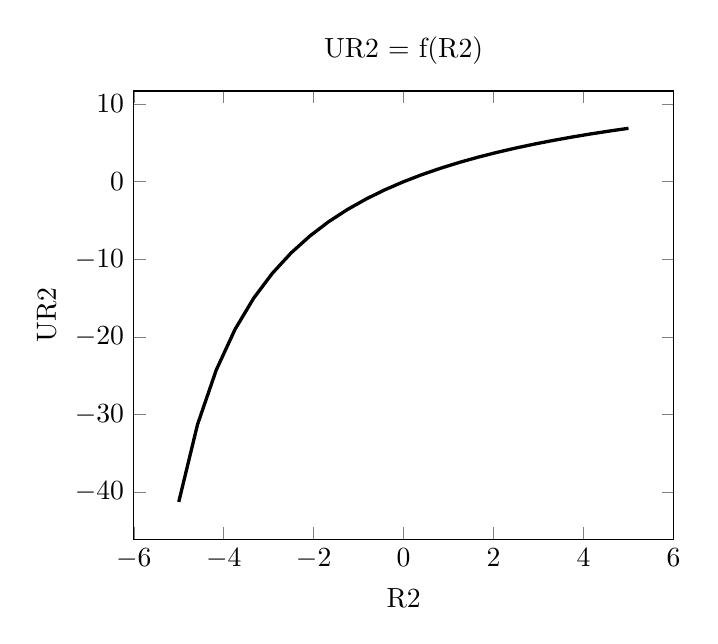
\begin{tikzpicture}
\begin{axis}[
    title = {UR2 = f(R2)},
    xlabel = R2,
    ylabel = UR2]
\addplot [black, very thick]{16.5*x/(7+x)};
\end{axis}
\end{tikzpicture}
\chapter{Praktiskā daļa}
\section{Darbs ar GEDA programmām}
\subsection{darbs ar gschem}
Ar GEDA komandu gschem es izveidoju vienkāršo shēmu (\ref{GEDA Shema})
\begin{figure}[!tb]
\includegraphics[width=\textwidth,height=\textheight,keepaspectratio]{01.png}
\caption{Elektriskā shēma no GEDA}
\label{GEDA Shema}
\end{figure}
\subsection{darbs ar gnetlist}
\begin{flushleft}
* Spice netlister for gnetlist  

V1 2 0 16.5  

R2 0 1 6  

R1 2 1 7  

.END  
  
\end{flushleft}
\subsection{darbs ar ngspice}
Ar ngspice es izveidoju divus grafikus. Att. (\ref{ngspice grafiks 1}) un (\ref{ngspice grafiks 2})
\begin{figure}[!tb]
\includegraphics[width=\textwidth,height=\textheight,keepaspectratio]{011.png}
\caption{Grafiks no ngspice (1)}
\label{ngspice grafiks 1}
\end{figure}
\begin{figure}[!tb]
\includegraphics[width=\textwidth,height=\textheight,keepaspectratio]{012.png}
\caption{Grafiks no ngspice (2)}
\label{ngspice grafiks 2}
\end{figure}
\section{Darbs are QUCS programmām}
\subsection{Principāla shēma}
\begin{figure}[!tb]
\includegraphics[width=\textwidth,height=\textheight,keepaspectratio]{02.png}
\caption{Principāla shēma}
\label{Principala shema}
\end{figure}
Shēma ar visiem elementiem, R2 ir aizvietots ar x lai to izmantot kā argumentu Parameter Sweep analīzē. (Att. \ref{Principala shema})
\subsection{Tabula un grafiks}
\begin{figure}[!tb]
\includegraphics[width=\textwidth,height=\textheight,keepaspectratio]{02_tabula_grafiks.png}
\caption{Tabula un grafiks}
\label{Tabula un grafiks}
\end{figure}
Kā ir redzams no grafika spriegums uz R2 mainās proporcionāli R2 pretestības izmaiņai pret kopējo pretestību. (Att. \ref{Tabula un grafiks})

\begin{thebibliography}{9}
\bibitem{gramata1}
Andrejs Strauts. Elektrotehnikas teorētiskie pamati, lekciju konspekts. –Rīga,
RTU, 2008, -197 lpp.
\bibitem{gramata2}
Kārlis Brīvkalns. Ķēžu teorija. Vadonis Ķēžu teorijas studijām: praktiskās
nodarbības, laboratorijas darbi, MatLab programmas,PSpice pielietojums. –Rīga,
RTU, 2008, - 93 lpp.
\end{thebibliography}
\end{document}
